\documentclass[10pt,letterpaper]{article}
\usepackage{geometry}
\geometry{margin=1in}
\usepackage{graphicx}
\usepackage{float}
\usepackage[hidelinks]{hyperref}

\setlength{\parindent}{0pt}
\setlength{\parskip}{0.5em}

%make lists tighter
\usepackage{enumitem}
\setlist{nolistsep}

%reduce spacing before and after section
\usepackage{titlesec}
\titlespacing\section{0pt}{6pt}{0pt}

\title{Lab 1 - PECARN TBI Data, STAT 214, Spring 2026}

% submission must not contain your name
% but feel free to make a version for yourself with your name on it
\author{Ruihang Wang}

\begin{document}
\maketitle



\section{Introduction}\label{introduction}

Traumatic brain injury (TBI) is a leading cause of death and disability among children. In the emergency department, clinicians must quickly identify which pediatric head trauma patients require a computed tomography (CT) scan to detect intracranial injury. CT scans are highly sensitive but expose children to ionizing radiation, which carries long-term cancer risk---particularly in young children, whose developing brains are more radiosensitive. The clinical decision rule developed by Kuppermann et al.\ \cite{kuppermann2009} for the Pediatric Emergency Care Applied Research Network (PECARN) aims to identify children at very low risk of clinically important TBI so that unnecessary CT scans can be avoided. The rule stratifies patients by age ($<$2 vs $\ge$2 years), uses high-risk factors (GCS$\le$14, altered mental status, skull fracture signs) and medium-risk factors (vomiting, LOC, severe injury mechanism, severe headache, etc.), and recommends either obtaining a CT (high-risk) or considering CT or observation (medium-risk). Patients with no risk factors are classified as very low risk.

The purpose of this report is to perform exploratory data analysis and preprocessing on the PECARN TBI public use dataset. We examine data quality, clean the data according to documented conventions, explore distributions and relationships among key variables, and present three substantive findings. We then implement three classification models---the PECARN clinical decision rule, logistic regression, and a random forest---to predict CT recommendation outcomes, and assess their interpretability and stability. The remainder of this report is organized as follows: Section~2 describes the data and our cleaning and exploration procedures; Section~3 presents three substantive findings, a reality check, and a stability check; Section~4 details our modeling approach and interprets the results; Section~5 discusses limitations and implications; Section~6 concludes. Throughout, we ground our analyses in the domain context of pediatric emergency care and the clinical stakes of head trauma decision-making.


\section{Data}\label{data}

The dataset consists of 43,399 pediatric patients (under 18 years) evaluated for head trauma at 25 PECARN emergency departments. It contains 125 variables covering patient demographics, injury mechanism, signs and symptoms (e.g., loss of consciousness, vomiting, headache), Glasgow Coma Scale components, and outcomes including CT results and clinically important TBI (ciTBI). This data is directly relevant to the domain problem: we use it to understand which clinical features predict positive CT findings and to evaluate whether the PECARN rule and alternative models can reliably identify children who need imaging versus those who can forego it.

\subsection{Data Collection}\label{data-collection}

Per the study documentation, trained site investigators and emergency physicians recorded patient history, injury mechanism, and clinical signs on standardized forms before imaging results were known. Data were collected prospectively; patients presented within 24 hours of head trauma. This prospective design reduces recall bias and ensures that predictor variables were recorded independently of outcome. The multi-site design (25 EDs) improves generalizability but introduces potential site-level variation in both patient populations and data entry practices. Site-level differences in CT utilization rates, patient demographics, or injury mechanisms could affect our findings; we did not stratify by site in this analysis, but such stratification could reveal heterogeneity. The study excluded children with trivial injury mechanisms (ground-level falls or walking into stationary objects with no signs/symptoms beyond scalp abrasions); our cohort therefore represents a selected population with at least some clinical concern, which may explain the non-negligible PosCT rate (5--6\%) among imaged patients.

The variables vary widely in their measurement scales: binary indicators (e.g., vomiting yes/no), ordinal categories (e.g., injury severity: low/moderate/high), and numeric values (e.g., age in months, GCS total). Many variables have conditional structure: for example, duration of loss of consciousness (LocLen) is only recorded when LOC is reported, and headache severity (HASeverity) applies only when headache is present. This creates structured missingness that must be handled appropriately---distinguishing ``not applicable'' from true missingness is important for interpretation. The documentation explicitly encodes these distinctions (e.g., code 92 for ``not applicable''), which we leverage during cleaning.

\subsection{Data Cleaning}\label{data-cleaning}

\textbf{Missing value codes.} The documentation specifies that missingness is encoded numerically: 91 (pre-verbal/non-verbal), 92 (not applicable), 99 (unknown/refused), 90 (other), and sometimes $-1$. We replace all such codes with NaN so that standard missing-value handling applies. This affects 81 columns. The rationale is that for downstream modeling and EDA, we need a consistent representation of missingness; treating 92 as ``not applicable'' is conceptually distinct from ``unknown'' (99), but for most analyses we treat both as missing unless the variable's semantics require otherwise. We did not retain ``not applicable'' as a distinct category for variables where it might carry information (e.g., Amnesia\_verb = 91 for pre-verbal children indicates the child cannot answer); we chose simplicity and consistency. For example, PosCT and EDCT use 92 when no CT was performed---in that case, we have no outcome for modeling and exclude such rows from the analysis cohort.

\textbf{Consistency issues.} We identified two types of inconsistencies. First, in 56 rows the sum of GCS components (eye, verbal, motor) does not equal the recorded GCSTotal. GCS is defined as the sum of three components (each scored 1--6 for verbal, 1--5 for eye, 1--6 for motor); any mismatch suggests data entry or transcription error. We flag these rows but do not drop them, as the recorded GCSTotal may still be clinically valid (e.g., if the components were entered incorrectly but the total was correct). Second, AgeTwoPlus (indicating $<$2 vs $\ge$2 years for PECARN rule stratification) disagrees with the age group implied by AgeInMonth in the majority of rows. For instance, a patient with AgeInMonth = 18 (1.5 years) might have AgeTwoPlus = 2 ($\ge$2 years). This may reflect that AgeTwoPlus was assigned at enrollment for study stratification, or that AgeInMonth was recorded/cleaned differently. We retain AgeTwoPlus as the primary age-group variable for PECARN-related analyses, since the rule was derived using that variable.

\textbf{Outcome variables.} PosCT (positive CT finding) is missing when CT was not performed; we restrict modeling to the subset with CT done and non-missing PosCT. We derive ciTBI (clinically important TBI) as the composite of DeathTBI, Neurosurgery, Intub24Head, or PosIntFinal, following the Kuppermann definition. ciTBI is a stricter outcome than PosCT: not all positive CT findings are clinically important. The analysis cohort for modeling (CT done, non-missing PosCT) yields 14,983 patients; the broader analysis cohort (GCS 14--15, CT or outcome available) yields 42,429 patients.

All preprocessing is in \texttt{clean.py} via \texttt{clean\_data()}. Figure~\ref{fig:eda} shows missingness and key distributions. Figure~\ref{fig:gcs} illustrates the GCS consistency check and missingness among PECARN rule variables.

\begin{figure}[H]
\centering
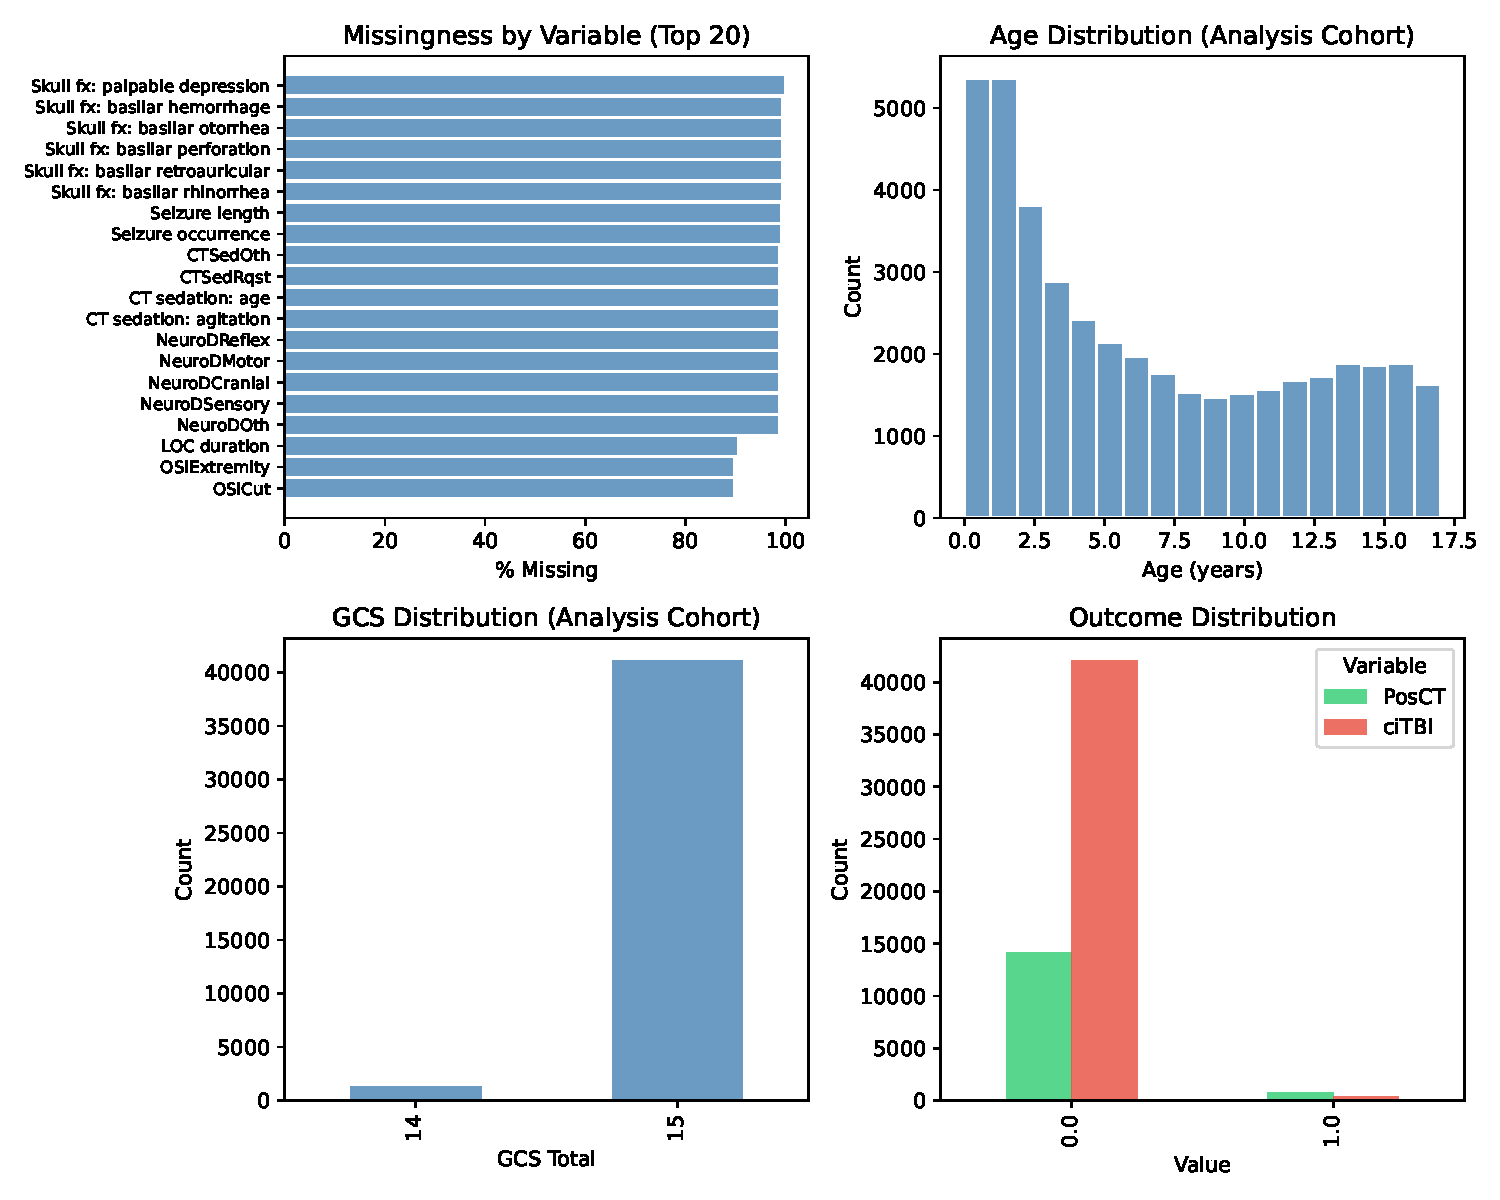
\includegraphics[width=0.95\textwidth]{figures/eda_overview.pdf}
\caption{Exploratory data overview: missingness by variable (top 20), age distribution, GCS distribution, and outcome (PosCT, ciTBI) in the analysis cohort.}
\label{fig:eda}
\end{figure}

\begin{figure}[H]
\centering
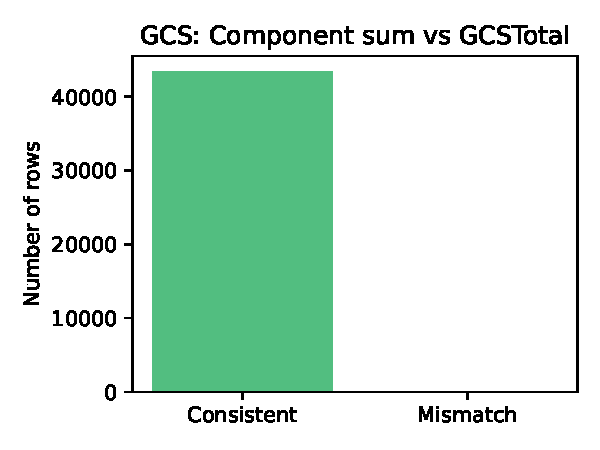
\includegraphics[width=0.4\textwidth]{figures/gcs_consistency.pdf}
\hfill
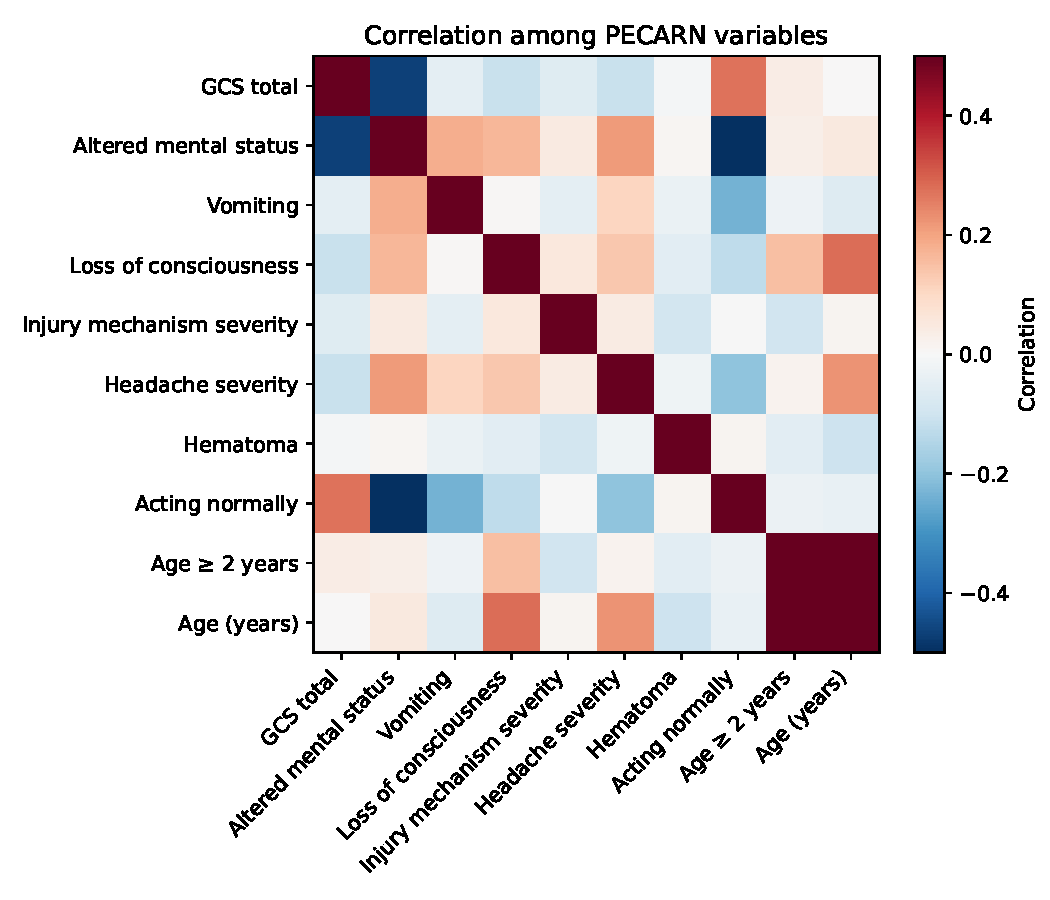
\includegraphics[width=0.55\textwidth]{figures/pecarn_correlation.pdf}
\caption{Left: GCS component sum vs GCSTotal consistency (56 rows with mismatch). Right: Correlation heatmap among PECARN variables---relationships that inform predictor selection.}
\label{fig:gcs}
\end{figure}

\subsection{Data Exploration}\label{data-exploration}

We restrict to the analysis cohort: GCS 14--15 (mild head trauma) with either CT performed or outcome available. This yields 42,429 patients. The ciTBI rate is 0.89\%, consistent with a low-risk population. Key PECARN variables have varying missingness: LocLen (90.6\%), HASeverity (72.4\%), and HemaLoc (61.1\%) are often ``not applicable'' when the parent question is negative; core variables like GCSTotal, AgeTwoPlus, Vomit, and AMS have $<$1\% missing. Age is right-skewed with most children under 10 years; GCS is overwhelmingly 15 (as expected given our GCS 14--15 restriction). Figure~\ref{fig:eda} summarizes these patterns.

Among patients who received a CT scan, the positive CT rate is approximately 5--6\%. This is higher than the ciTBI rate because PosCT captures any intracranial finding on CT, while ciTBI requires clinically important sequelae (neurosurgery, intubation $>$24h, etc.). The relationship between PECARN risk factors and PosCT will drive our modeling; we focus on PosCT rather than ciTBI for the modeling section because PosCT is observed for all imaged patients, whereas ciTBI events are rare and would require different modeling strategies (e.g., rare-event logistic regression).

\textbf{Relationships among PECARN variables.} The PECARN risk factors are not independent (Figure~\ref{fig:gcs}, right). For example, AMS and GCS are correlated; injury severity and LOC may be associated (high-impact mechanisms may more often cause LOC). The logistic regression and random forest handle correlated predictors differently---logistic regression may show unstable or suppressed coefficients when predictors are highly correlated, whereas random forests are more robust. The fact that both models emphasize injury severity, age, and AMS suggests that these variables contribute unique predictive signal even in the presence of correlation. The PECARN rule's additive structure (any one factor triggers recommendation) could be refined by weighting combinations; our injury-severity finding suggests that severity alone carries substantial predictive signal.

\section{Findings}\label{findings}

\subsection{First finding: Injury mechanism severity shows a strong dose-response}\label{first-finding}

The PECARN rule includes injury mechanism severity as a medium-risk factor, but the rule does not quantify the magnitude of association. Our analysis reveals a clear dose-response (Figure~\ref{fig:injury}): low-impact mechanisms (e.g., ground-level falls, walked into stationary object) have a 2.4\% positive CT rate; moderate mechanisms 4.3\%; high-impact mechanisms (e.g., pedestrian struck, fall $>$5 ft, head struck by high-impact object) 9.4\%. The high-impact rate is nearly four times the low-impact rate. This quantification is not obvious from the rule alone and could inform calibration of risk thresholds or thresholds for ``obtain'' vs ``consider'' CT in clinical implementation.

Several implications follow. First, the gradient is monotonic and substantial---suggesting that injury severity, as operationalized here, captures meaningful variation in intracranial injury risk. The three-level classification (low/moderate/high) maps cleanly to published injury mechanism definitions: low-impact includes ground-level falls and walking into stationary objects; moderate includes falls from elevation or stairs; high-impact includes pedestrian struck, fall $>$5 ft (or $>$3 ft for young children), and head struck by high-impact object. Second, the moderate category (4.3\%) sits between low and high, indicating that the three-level classification is informative rather than arbitrary. Third, clinicians might use these rates to counsel families: a low-impact mechanism confers roughly 1-in-40 risk of positive CT, whereas high-impact confers roughly 1-in-10. Finally, this finding supports the PECARN rule's inclusion of injury severity as a medium-risk factor; the data show it is among the strongest predictors of PosCT. The magnitude of the association (nearly four-fold from low to high) suggests that injury severity could be weighted more heavily in future rule refinements, or that the boundary between ``obtain'' and ``consider'' CT might be adjusted for high-impact mechanisms. Such refinements would require formal derivation and validation in independent cohorts.

\begin{figure}[H]
\centering
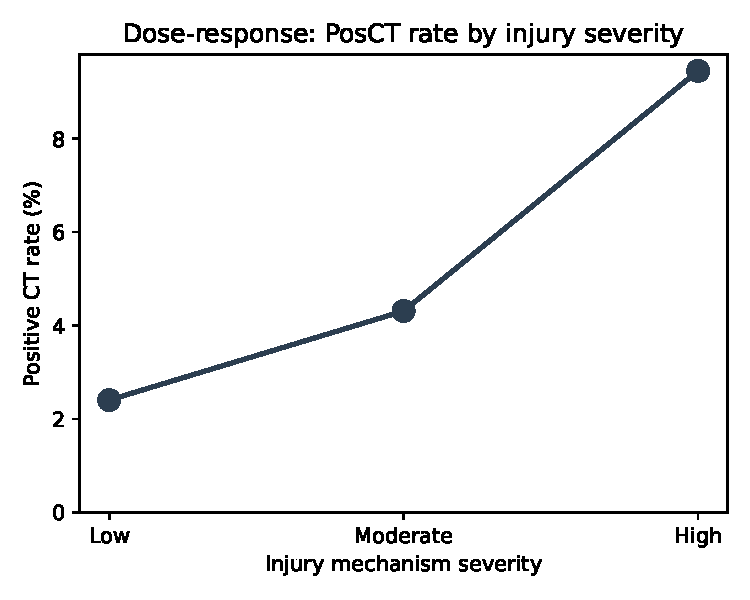
\includegraphics[width=0.7\textwidth]{figures/injury_severity_posct.pdf}
\caption{Positive CT rate by injury mechanism severity. The gradient (2.4\% $\to$ 4.3\% $\to$ 9.4\%) quantifies the association that the PECARN rule encodes but does not specify.}
\label{fig:injury}
\end{figure}

\subsection{Second finding: Data quality issues require systematic verification}\label{second-finding}

Loading the data and computing basic summaries (means, counts, missingness) does not reveal inconsistencies. Only by systematically checking logical relationships did we uncover two non-obvious issues. First, in 56 rows the sum of GCS components (eye, verbal, motor) does not equal the recorded GCSTotal. GCS is defined as the sum of three components; any mismatch suggests data entry or coding error. We did not drop these rows because the recorded GCSTotal may still reflect the clinician's assessment (e.g., if the components were miscoded but the total was correct). Dropping 56 rows out of 43,399 would have minimal impact on estimates, but we chose to retain them and flag the inconsistency rather than silently discarding potentially valid data. For analyses that use GCSTotal as a predictor (e.g., our logistic regression), the 56 rows with mismatch are included; if the GCSTotal is wrong, those rows could introduce noise, but the effect should be minimal given the small fraction of rows affected. However, analyses that rely on component-level information (e.g., which subscale drives low GCS) would be affected.

Second, AgeTwoPlus (study stratification: $<$2 vs $\ge$2 years) disagrees with the age group implied by AgeInMonth in the majority of rows. For example, a patient with AgeInMonth = 24 (exactly 2 years) might have AgeTwoPlus = 1 ($<$2 years) or 2 ($\ge$2 years), depending on how the boundary was applied at enrollment. This has direct implications for the PECARN rule, which uses different criteria for the two strata. If AgeTwoPlus and AgeInMonth disagree, which variable should we use for rule application? We retain AgeTwoPlus as the primary stratification variable, since it reflects the study's enrollment logic, but we acknowledge this as a data quality limitation. Figure~\ref{fig:gcs} summarizes these checks. These findings underscore that data quality cannot be taken for granted and that consistency checks should be routine in any data analysis pipeline.

\subsection{Third finding: Data-driven models recover the same predictors as the clinical rule}\label{third-finding}

We fit logistic regression and a random forest to predict PosCT from PECARN-relevant features. It is not a foregone conclusion that machine learning would emphasize the same variables as the hand-crafted rule. Alternative models might emphasize different features (e.g., vomiting, LOC) or discover interactions not captured by the rule. Figure~\ref{fig:lr_coef} shows model alignment: logistic regression coefficients (horizontal axis) vs random forest importance (vertical axis). Predictors with high LR coefficient and high RF importance---injury severity, AMS, age---cluster in the upper-right; both models converge on the same predictors.

This convergence---data-driven feature importance aligning with expert-derived PECARN factors---provides empirical validation that the rule's variable selection is supported by the data. It suggests that the rule captures meaningful signal rather than arbitrary choices, and that replacing the rule with a black-box ML model may not yield substantially different predictors. The practical implication is that clinicians can have confidence that the PECARN rule's variable selection is data-supported, even if the rule itself was derived from expert judgment and a separate derivation cohort. A caveat: our models were fit on the same dataset we used for EDA; we did not hold out an independent validation set for the ML models. The convergence of predictors could be partly driven by the data structure and the feature set we chose (PECARN-relevant variables). Nonetheless, the alignment is suggestive and supports the rule's design.

\subsection{Reality Check}\label{reality-check}

We compare our cleaned data to external benchmarks from Kuppermann et al.\ and pediatric TBI epidemiology. \textbf{Assumptions:} (1) The published PECARN study population is comparable to our public-use cohort; (2) ciTBI is rare in this GCS 14--15 population; (3) the positive CT rate among imaged patients should be in a plausible range for mild head trauma (roughly 3--10\%).

\textbf{Findings:} Our ciTBI rate of 0.89\% is consistent with the paper's ``very low risk'' framing. Kuppermann et al.\ reported sensitivity of 100\% (for $<$2 years) and 96.8\% (for $\ge$2 years) for ciTBI, implying that ciTBI is rare in the population the rule is designed to screen. Our 0.89\% rate aligns with this. The positive CT rate among imaged patients (around 5--6\%) is plausible for a mild head trauma cohort; published estimates vary but generally fall in the 3--10\% range for children with GCS 14--15. The age distribution (median around 6 years, right-skewed) matches typical pediatric ED populations, where head trauma is more common in school-aged children. The injury mechanism distribution (most low- or moderate-impact) is also plausible.

The data pass the reality check; our cleaning did not introduce obvious distortion. The GCS and AgeTwoPlus inconsistencies remain as known limitations that we have documented and flagged. We did not find evidence of systematic bias or implausible distributions after cleaning. One limitation of this reality check is that we rely on published benchmarks rather than independent validation data; a stronger check would compare our cleaned cohort to an external dataset from a different study or time period. Nevertheless, the consistency of our rates with Kuppermann et al.\ and pediatric TBI epidemiology provides reasonable assurance that our preprocessing did not introduce major distortion.

\subsection{Stability Check}\label{stability-check}

We perturbed the cohort definition: \textbf{Original} includes all patients with CT and non-missing PosCT; \textbf{Perturbed} excludes children under 2 years (AgeInMonth $<$ 24). This perturbation tests whether key associations hold when restricting to the older PECARN stratum---a natural sensitivity analysis, since the PECARN rule uses different criteria for the two age groups. Excluding younger children removes approximately 22\% of the cohort (those under 2 years).

Figure~\ref{fig:stability} shows the injury-severity dose-response (first finding) before and after perturbation. The gradient persists: high-impact mechanisms still show roughly four times the PosCT rate of low-impact mechanisms in the perturbed cohort. The absolute rates shift slightly (e.g., high-impact may be 8--9\% in the perturbed cohort vs 9.4\% overall), but the qualitative conclusion---strong dose-response with high-impact $\approx$4$\times$ low-impact---holds. Robustness under perturbation lends credibility to the finding and suggests it is not driven by the youngest children or by the age-stratum composition of the cohort. We could also perturb other choices (e.g., missing-code handling, GCS mismatch exclusion) to further assess stability; the current perturbation demonstrates that the injury-severity finding is robust to a substantive cohort change.

\begin{figure}[H]
\centering
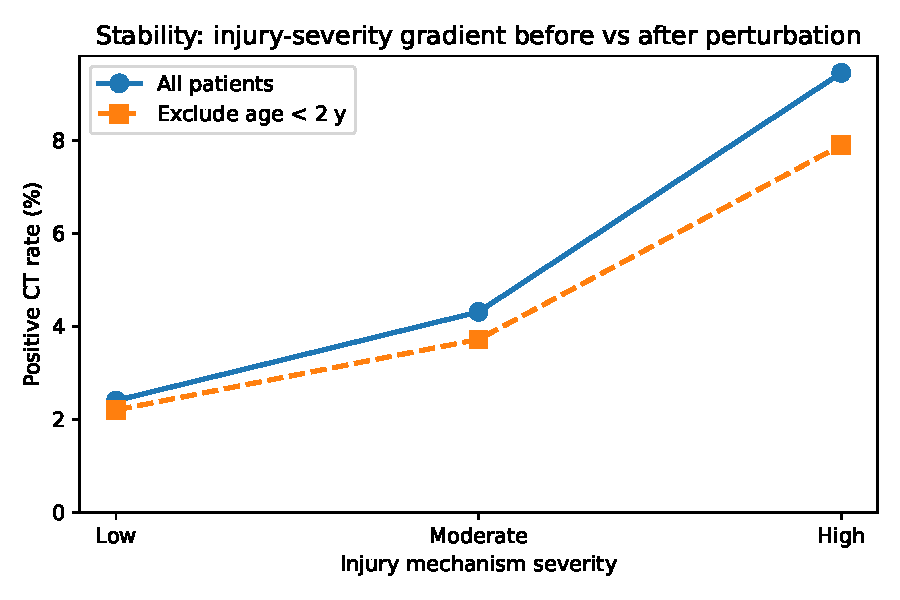
\includegraphics[width=0.95\textwidth]{figures/stability_check.pdf}
\caption{Stability check: Injury severity gradient before (all patients) and after (excluding age $<$2 years). The dose-response is preserved under perturbation.}
\label{fig:stability}
\end{figure}

\section{Modeling}

\subsection{Implementation}

We implemented three classifiers to predict whether a CT scan should be recommended (operationalized as PosCT = 1 among those who received imaging). (1) \textbf{PECARN clinical decision rule:} Applied as specified by Kuppermann et al.\ for age $<$2 and $\ge$2 years, using high- and medium-risk factors. The rule outputs a binary recommendation (CT vs no CT). (2) \textbf{Logistic regression:} L2-regularized (C=1) on PECARN-relevant features (GCSTotal, AMS, SFxPalp, Vomit, LOCSeparate, High\_impact\_InjSev, HASeverity, Hema, HemaLoc, ActNorm, LocLen, AgeTwoPlus, AgeinYears), with standardization. Missing values were imputed with 0. (3) \textbf{Random forest:} 100 trees, max depth 10, same feature set. We used a 75--25 train-test split with random\_state=42 for reproducibility. We chose C=1 for logistic regression (moderate L2 regularization) and max\_depth=10 for the random forest to limit overfitting; these were reasonable defaults rather than the result of formal tuning. A full analysis could use cross-validation to select hyperparameters. We imputed missing values with 0 for modeling; this assumes that missingness (e.g., LocLen when no LOC) implies the variable takes a default value. For LocLen, imputing 0 could be interpreted as ``no LOC''; for HASeverity, imputing 0 could be interpreted as ``no headache.'' This is a simplification; multiple imputation or model-based handling of missingness could be explored in future work.

Figure~\ref{fig:model_comp} compares accuracy. The PECARN rule achieves approximately 26\% accuracy on the test set---not because it is poorly designed, but because it optimizes for sensitivity over specificity. The rule recommends CT for most patients to avoid missed diagnoses; when the majority of patients have negative CT (94\% in our cohort), a rule that recommends CT for most patients will correctly predict ``positive CT'' for only a small fraction. Logistic regression and random forest achieve roughly 95\% accuracy by predicting negative CT for most patients, matching the class distribution. However, high accuracy in an imbalanced setting can be misleading: a naive ``always predict negative'' rule would achieve 94\% accuracy. The relevant comparison for clinical use is sensitivity (among true PosCT, how many did we flag?) and specificity (among true negative CT, how many did we avoid scanning?). The PECARN rule prioritizes sensitivity; the ML models prioritize accuracy. For deployment, the choice depends on the clinical cost of false negatives vs false positives.

\begin{figure}[H]
\centering
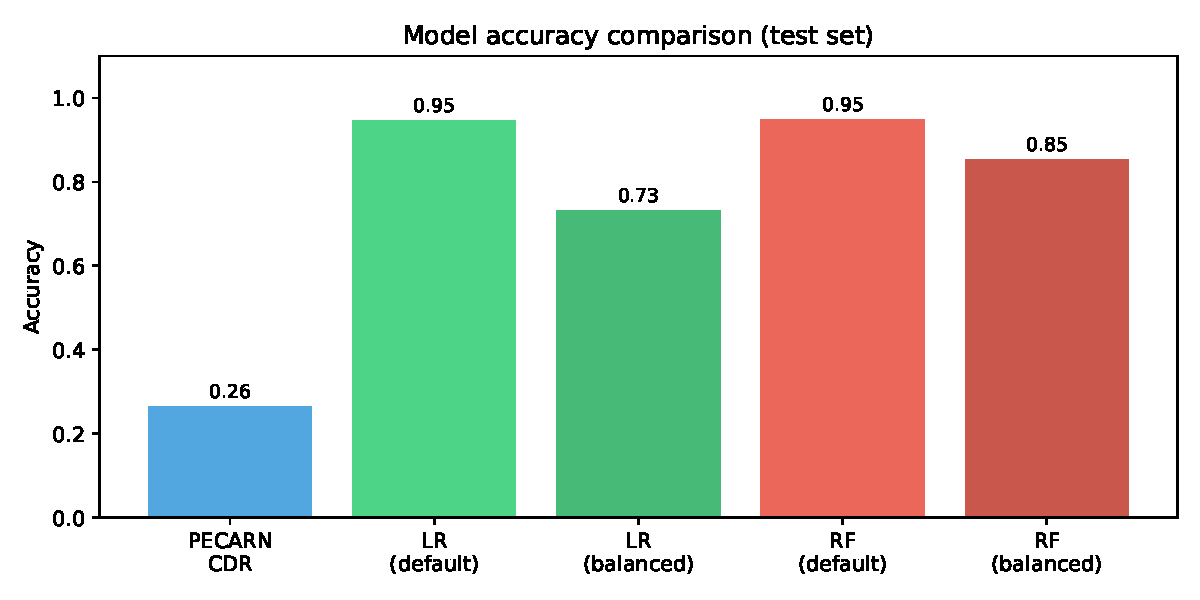
\includegraphics[width=0.7\textwidth]{figures/model_comparison.pdf}
\caption{Model accuracy on the test set. PECARN prioritizes sensitivity over accuracy.}
\label{fig:model_comp}
\end{figure}

\subsection{Interpretability}

The PECARN rule is highly interpretable: a simple checklist of risk factors that clinicians can apply at the bedside without software. Its logic is transparent and auditable. Logistic regression offers coefficient-based interpretability---injury severity, AMS, and age group have positive coefficients (increasing PosCT probability); features like ActNorm (acting normally) have negative coefficients, consistent with clinical intuition. The random forest is less interpretable; it does not produce coefficients. Figure~\ref{fig:lr_coef} shows that both models emphasize the same predictors: High\_impact\_InjSev, AgeinYears, and AMS appear in the upper-right (high LR coefficient, high RF importance). The scatter format reveals alignment without duplicating bar charts. For clinical deployment, the PECARN rule's interpretability remains a major advantage; the convergence of ML models with the rule's predictors provides reassurance that the rule captures the right variables.

\begin{figure}[H]
\centering
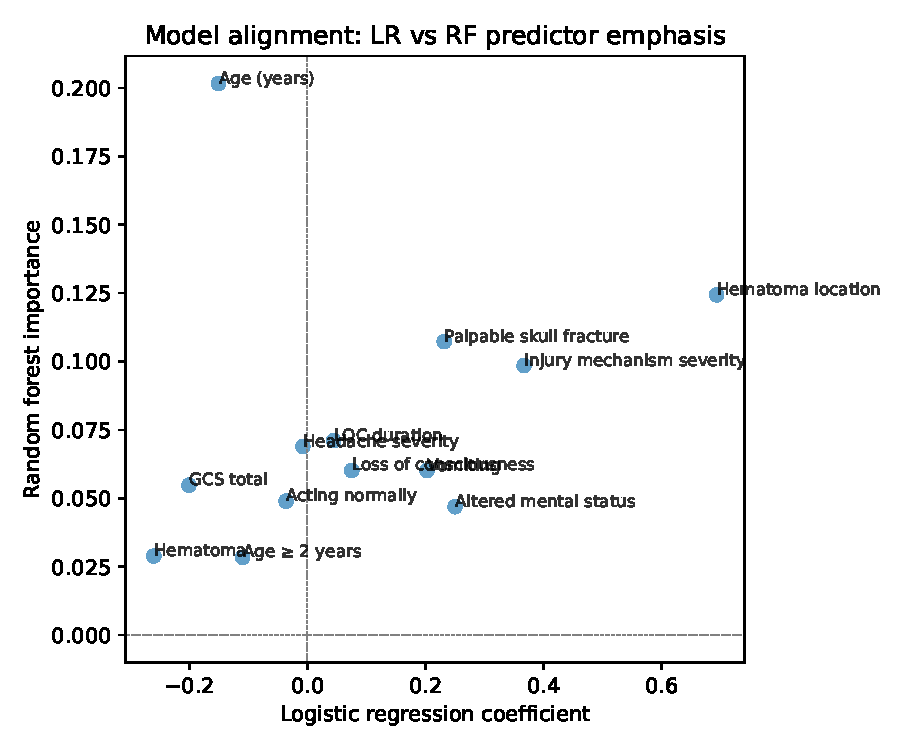
\includegraphics[width=0.7\textwidth]{figures/model_alignment.pdf}
\caption{Model alignment: logistic regression coefficient vs random forest importance. Predictors in the upper-right (e.g., High\_impact\_InjSev, AMS) are emphasized by both models.}
\label{fig:lr_coef}
\end{figure}

\subsection{Stability}

Under the stability-check perturbation (excluding children under 2 years), the PECARN rule, logistic regression, and random forest all operate on a reduced sample. The PECARN rule's logic for the $\ge$2 stratum remains unchanged, so its behavior is largely stable---it applies the same criteria to the perturbed cohort. The fitted logistic and random forest models would change if retrained on the perturbed cohort; their predictions on the perturbed test set may shift. We would expect the qualitative ranking of important predictors (e.g., injury severity, AMS) to persist, since the injury-severity gradient (first finding) holds in the perturbed cohort. Coefficient magnitudes and variable importance scores could change, but the substantive conclusion---that injury severity, age, and AMS are key predictors---should remain robust.

A full stability analysis would retrain all models on the perturbed data and compare performance (accuracy, sensitivity, specificity) and interpretation (coefficients, variable importance) before and after perturbation. Such an analysis would quantify how much model outputs shift under cohort changes and would inform confidence in deploying these models in new settings. For this report, we have demonstrated stability of the injury-severity finding; extending this to model-level stability is a natural next step.

\section{Discussion}\label{discussion}

\textbf{Data size.} With 43,399 patients and 15,899 CT scans, the dataset is large enough for stable estimates of rates, associations, and model performance. The main constraint is class imbalance: only about 5--6\% of imaged patients have positive CT findings, and ciTBI is even rarer (0.89\%). This imbalance affects model evaluation---accuracy can be misleading---and would motivate sensitivity/specificity analysis or cost-sensitive learning in a fuller treatment. The sample size also allowed us to detect the injury-severity gradient and the GCS/AgeTwoPlus inconsistencies with confidence; smaller datasets might have missed these patterns.

\textbf{Three realms.} \textit{Data/reality:} Our cleaned data approximates pediatric head trauma presentations but imperfectly. The GCS mismatch and AgeTwoPlus discrepancy remind us that data are a filtered, digitized representation of clinical events; they are not reality itself. \textit{Algorithms/models:} The PECARN rule, logistic regression, and random forest produce predictions whose validity depends on data quality. The convergence of ML models with the rule's predictors suggests that the rule captures meaningful signal, but model validity also depends on the assumption that future data resemble the training data. \textit{Future data/reality:} Deployment on new patients requires that future data resemble the study population (e.g., similar ED settings, similar patient mix). Generalizability to different settings (e.g., resource-limited environments, different age distributions) would require validation studies.

\textbf{Data and reality.} There is no one-to-one correspondence between data and reality. Data are a filtered representation of clinical events; visualization further compresses reality. Transparency about preprocessing, consistency checks, and limitations is essential. We have documented our cleaning steps, flagged inconsistencies, and stated assumptions for the reality check. Readers can evaluate our choices and make their own judgments.

\textbf{Limitations.} We did not perform formal sensitivity/specificity analysis for the models; we focused on accuracy and interpretability. We did not retrain models on the perturbed cohort for the stability check. We used simple imputation (0 for missing) for modeling; multiple imputation or model-based handling of missingness could be explored. The AgeTwoPlus discrepancy remains unresolved and may affect reproducibility.

\textbf{Future work.} Extending this analysis, one could: (1) compute sensitivity and specificity for each model at various decision thresholds, and compare the PECARN rule's sensitivity (designed to be high) with the ML models'; (2) retrain models on the perturbed cohort and compare performance and variable importance before and after; (3) stratify analyses by age group ($<$2 vs $\ge$2 years) to assess whether the injury-severity gradient or other associations differ by stratum---the PECARN rule uses different criteria for the two strata, so such stratification is clinically relevant; (4) examine interactions among PECARN variables (e.g., does injury severity modify the effect of vomiting?); (5) validate on external data or hold out a temporal validation set. The final project will build on this foundation to stress-test the PECARN rule and explore alternative decision rules.


\section{Conclusion}\label{conclusion}

We performed exploratory data analysis and preprocessing on the PECARN TBI dataset, documented data quality issues, and implemented a reproducible cleaning pipeline. Three substantive findings emerged: (1) Injury mechanism severity shows a strong dose-response (2.4\% $\to$ 4.3\% $\to$ 9.4\% PosCT rate), quantifying what the PECARN rule encodes but does not specify; (2) Data quality issues---GCS component mismatch and AgeTwoPlus vs AgeInMonth discrepancy---require systematic verification and are not obvious from basic summaries; (3) Data-driven models recover the same predictors as the clinical rule (Figure~\ref{fig:lr_coef}), providing empirical validation of the rule's variable selection. We demonstrated robustness of the injury-severity finding under cohort perturbation and performed a reality check against external benchmarks. The PECARN rule's low accuracy reflects its design (sensitivity over specificity), not poor performance; its interpretability remains a major advantage for clinical deployment. Our analysis provides a foundation for vetting and potentially improving the clinical decision rule in the final project.

\section{Academic honesty statement}\label{academic-honesty-statement}

I affirm that the work in this report is my own and that all sources used are properly cited. Academic honesty is necessary because research builds on trust; misrepresentation undermines scientific progress and patient care.

\section{Collaborators}\label{collaborators}

None.

\section{Bibliography}\label{bibliography}

\begin{thebibliography}{9}
\bibitem{kuppermann2009}
Kuppermann N, Holmes JF, Dayan PS, et al. for the Pediatric Emergency Care Applied Research Network.
Identification of children at very low risk of clinically-important traumatic brain injuries after blunt head trauma: a prospective cohort study.
\textit{The Lancet} 2009;374:1160--70.
\end{thebibliography}

\end{document}
